\documentclass[amscd, amssymb, verbatim]{amsart}[12pt]

\usepackage{amsmath,amssymb,amsthm}
\usepackage[utf8]{inputenc}
\usepackage{graphicx}
\usepackage{fullpage}
\usepackage[colorlinks,linkcolor=blue,urlcolor=blue,citecolor=blue,destlabel=true]{hyperref}
\usepackage{placeins}

\newcommand{\note}[1]{\textcolor{blue}{({#1})}}

\theoremstyle{plain}
\newtheorem{lemma}{Lemma}[section]
\newtheorem{theorem}[lemma]{Theorem}
\newtheorem{fact}[lemma]{Fact}
\newtheorem{corollary}[lemma]{Corollary}
\newtheorem{proposition}[lemma]{Proposition}
\newtheorem{conjecture}[lemma]{Conjecture}
\newtheorem{problem}[lemma]{Problem}
\newtheorem{claim}[lemma]{Claim}
\theoremstyle{definition}
\newtheorem{definition}[lemma]{Definition}
\newtheorem{example}[lemma]{Example}
\newtheorem{question}[lemma]{Question}
\newtheorem{remark}[lemma]{Remark}

\newcommand{\N}{\mathbb{N}}
\newcommand{\R}{\mathbb{R}}
\newcommand{\Z}{\mathbb{Z}}
\newcommand{\cB}{\mathcal{B}}
\newcommand{\cone}{\mathrm{Cone}}
\DeclareMathOperator{\cl}{Cl}

\begin{document}

\title{On the minimal cores of unit disk graphs}
\author{CSU Putnam Seminar, Spring 2019}
\date{\today}
\maketitle

\note{You can type any comments or ask questions in a blue ``note" environment!}


\section{Project Overview}

The wikipedia article \url{https://en.wikipedia.org/wiki/Cop-win\_graph} explains a game of pursuit evasion on a graph $G$, where a robber is trying to evade a cop. 
We say that a graph $G$ is \emph{cop-win} if, no matter where the cop and robber are placed initially, the cop can always catch the robber.

It turns out that a graph $G$ is a cop-win graph if and only if it is \emph{dismantlable}, which we will describe in Section~\ref{sec:cop-win}.
Roughly speaking, a graph is dismantlable if you can ``remove dominated vertices" until you end up with only a single vertex.
More generally, after you have removed as many dominated vertices as possible, the resulting graph is called a \emph{minimal core}. Surprisingly, it turns out that all possible minimal cores of a graph are isomorphic to each other.

In this project, we will study the minimal cores of unit disk graphs.
A unit disk graph is a very particular type of graph which is formed by selecting a finite set of vertices in the plane $\R^2$, and then connecting two vertices by an edge if and only if the Euclidean distance between them is at most one.

The minimal cores of unit disk graphs from points on the circle are already classified.
Roughly speaking, one of our main questions will be to explore whether unit disk graphs from points in $\R^2$ are ``simple combinations" of unit disk graphs from points on the circle, or if the unit disk graphs from arbitrary points in $\R^2$ can exhibit ``wildly new phenomena."

One of our first tasks will be to learn the basics of cop-win graphs.

A major task will be to write software that can accept an arbitrary graph as input, and then as output return a minimal core.
We can test this software on unit disk graphs from the circle.
We will then use this software to visualize unit disk graphs of points in $\R^2$.

A later task will be to learn a little bit of combinatorial topology.
Part of the motivation for this project is to prove or disprove the conjecture that ``the clique complex of the unit disk graph of any finite set of points in $\R^2$ is always homotopy equivalent to a wedge sum of spheres", whatever in the world that means!

\section{Introduction}

\section{Cop-win graphs}\label{sec:cop-win}

Let $G=(V,E)$ be a simple undirected graph (no loops or multiple edges) with $V$ the set of vertices and with $E$ the set of edges.

For any vertex $v\in V$, let $N[v]=\{v\}\cup\{u\in V~|~uv\in E\}$ be the \emph{closed neighborhood} of $v$ (where ``closed" implies that the vertex $v$ is itself included in this neighborhood).
\begin{definition}\label{def:dominated}
In a graph $G$, we say that a vertex $v$ is \emph{dominated} by a vertex $u$ if $N[v]\subseteq N[u]$.
\end{definition}

\begin{figure}[h]
\centering
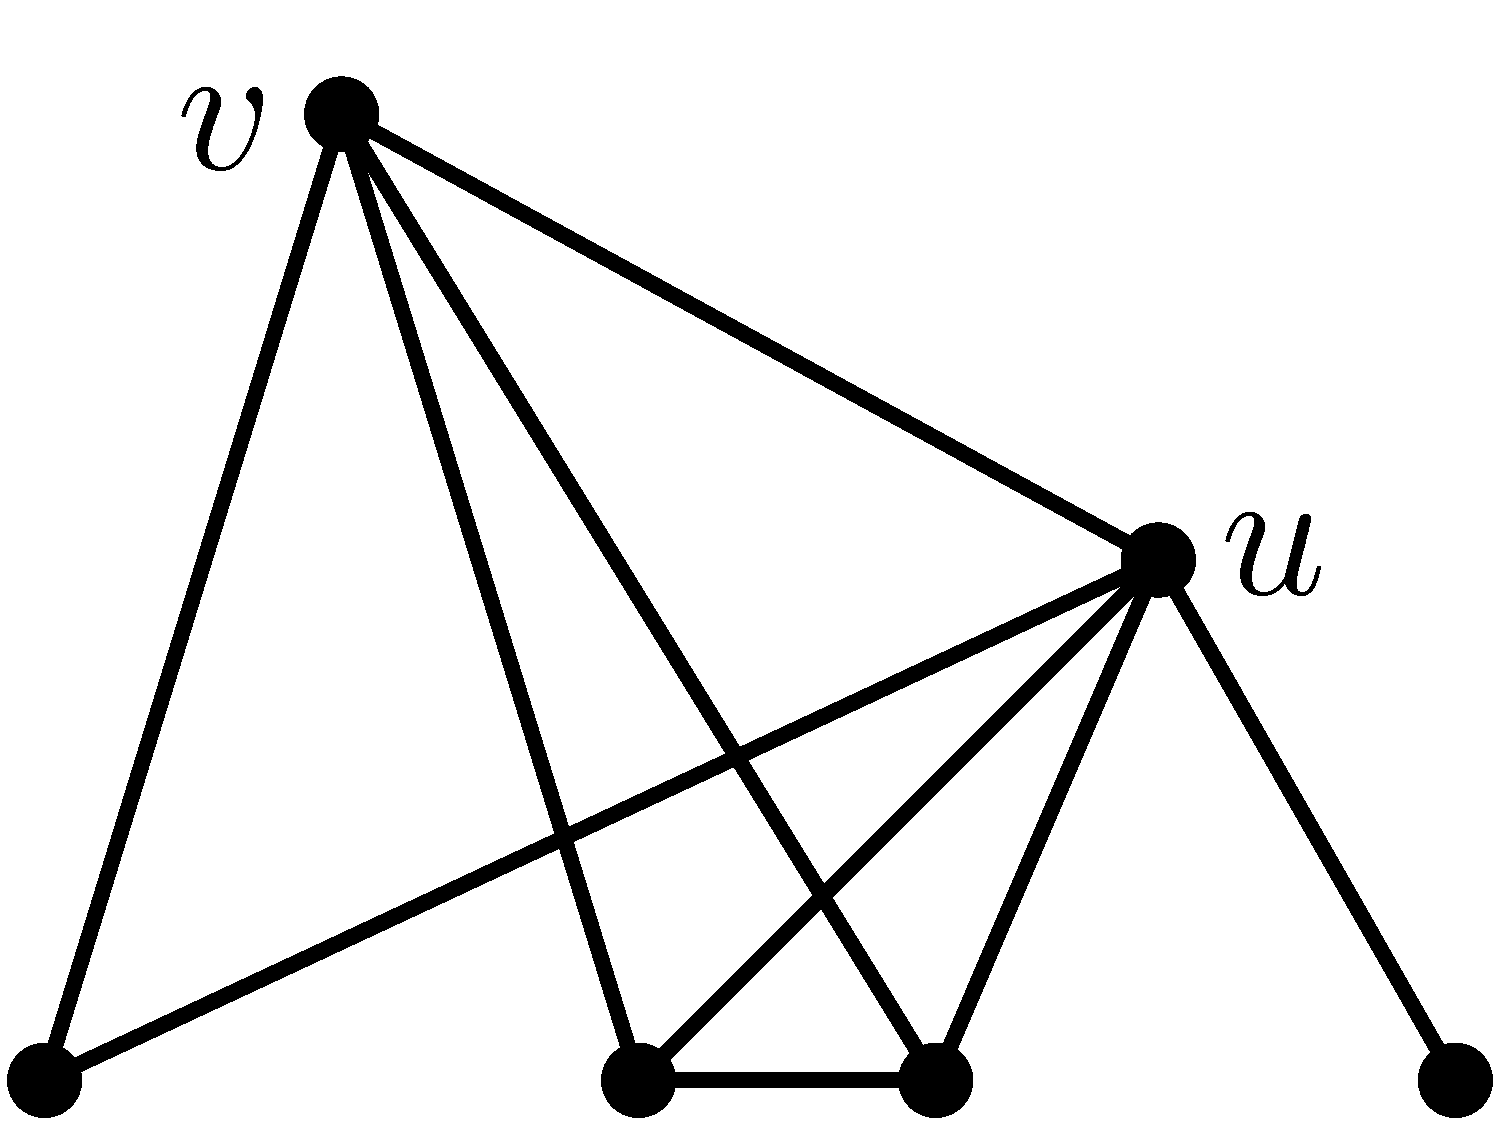
\includegraphics[width=0.2\textwidth]{Dominated1_labeled.pdf}
\caption{Vertex $v$ is dominated by vertex $u$.}
\label{fig:dominated}
\end{figure}

%Let $G\setminus u$ be the graph obtained by deleting $u$ and all of the edges containing $u$.

If you iteratively remove dominated vertices from a graph $G$, then your final ending configuration (once there are no more remaining dominated vertices) is called a \emph{minimal core}.
Surprisingly, all minimal cores of a graph are isomorphic.

We say that a graph $G$ is \emph{dismantlable} if its minimal core is a single vertex, or equivalently, if one can remove dominated vertices one-by-one until only a single vertex remains.
A cool theorem is that a graph is a cop-win graph if and only if it is dismantlable.



\section{Algorithms for computing minimal cores}
See \url{https://en.wikipedia.org/wiki/Cop-win\_graph} for some information on algorithms computing the minimal core of a graph.
What software options are out there, and should we write our own?
The main place to look is google!
Two other places to look are sage and polymake.

I claim that if we wish to implement it ourselves, the ``right'' way to do it is to implement the graph data structure in \url{https://www.sciencedirect.com/science/article/pii/S0304397511009662?via\%3Dihub}, because it will help time bounds greatly for finding dominated vertices.  It does look kinda complicated, but that paper has everything we would need. 

\note{Todo Henry: Share a mathematica demo for Vietoris--Rips complexes!}

% Useless trivia: If you remove a dominated vertex from a graph, no dominated vertices will become un-dominated.  However, new dominated vertices \emph{may} be created.  Thus, a simple greedy algorithm (e.g. while there exists a dominated vertex, remove it) will not return incorrect results.


\section{Unit disk graphs}



\section{Minimal cores of unit disk graphs on the circle}

\note{These are classifiable---Henry will describe.}



\section{Minimal cores of unit disk graphs in the plane}

\note{This is where we will be doing much of our exploring/work!}



\section{Questions}

Are the minimal cores of unit disk graphs in the plane ``simple cominations" of unit disk graphs from points on the circle, or can they exhibit ``wildly new phenomena"?



\section{Related references}

Related references for the non-topological aspects of this project include the following.
The original paper appears to be~\cite{aigner1984game}, available at (\footnote{\url{https://www.math.ucdavis.edu/~erikslivken/classes/2016\_spring\_180/aigner\%20fromme.pdf}}). There is also a book~\cite{bonato2011game} by the author of (\footnote{\url{http://www.math.ryerson.ca/~abonato/papers/conjectures\_CR\_jan18\_2015.pdf}}). See the webpages (\footnote{\url{https://users.auth.gr/kehagiat/Research/CopRob/index.htm}}), (\footnote{\url{http://math.ucsd.edu/~fan/152/arch/coprob/}}), (\footnote{\url{https://www.mathworks.com/matlabcentral/fileexchange/31774-cops-and-robber-software}}), and the references within. See also (\footnote{\url{https://arxiv.org/pdf/1108.2549.pdf}}), (\footnote{\url{https://www.cambridge.org/core/journals/combinatorics-probability-and-computing/article/cops-and-robbers-on-geometric-graphs/22DA76A41397162164E755B52D6C3D81}}), (\footnote{\url{https://www.universiteitleiden.nl/binaries/content/assets/science/mi/scripties/master/2017-2018/mark-van-den-bergh-08-09-2017.pdf}}).



\newpage


\section{The topological perspective}

Recall that a graph is a collection of vertices (0-dimensional pieces) and edges (1-dimensional pieces) that are ``glued-together compatibly".
What if we now also allow triangles (2-dimensional pieces), tetrahedra (3-dimensional pieces), etc? The resulting object is called a \emph{simplicial complex}; see for example \url{https://en.wikipedia.org/wiki/Simplicial\_complex}. 
Instead of calling these pieces vertices, edges, triangles, tetrahedra, etc, we can more efficiently call them $k$-simplices, where $k$ is the dimension of the piece!
For example, a vertex is a 0-simplex, an edge is a 1-simplex, a triangle is a 2-simplex, and a tetrahedron is a 3-simplex. Note that a $k$-simplex is a $k$-dimensional building block consisting of $k+1$ vertices. The advantage of this notation is that now we can also talk about $k$-simplices for any $k\ge 0$!
Though some definitions of simplicial complexes feel a little abstract, the right perspective is to think of a simplicial complex as a LEGO set that is formed by gluing simple building blocks (simplices) together!

\begin{definition}
A \emph{simplicial complex} $K$ on a vertex set $V$ is a set of simplices $\sigma \subseteq V$, such that if $\sigma\in K$ (meaning $\sigma$ is a simplex in the complex) and $\tau\subseteq\sigma$ (meaning $\tau$ is a face of $\sigma$), then we also have $\tau\in K$ (meaning that $\tau$ is also a simplex in the complex).
\footnote{Strictly speaking, if we we want to say that $V$ is the vertex set of $K$, then we should also specify that each singleton element of $V$ is a simplex in $K$.}
\end{definition}

\begin{figure}[h]
\centering
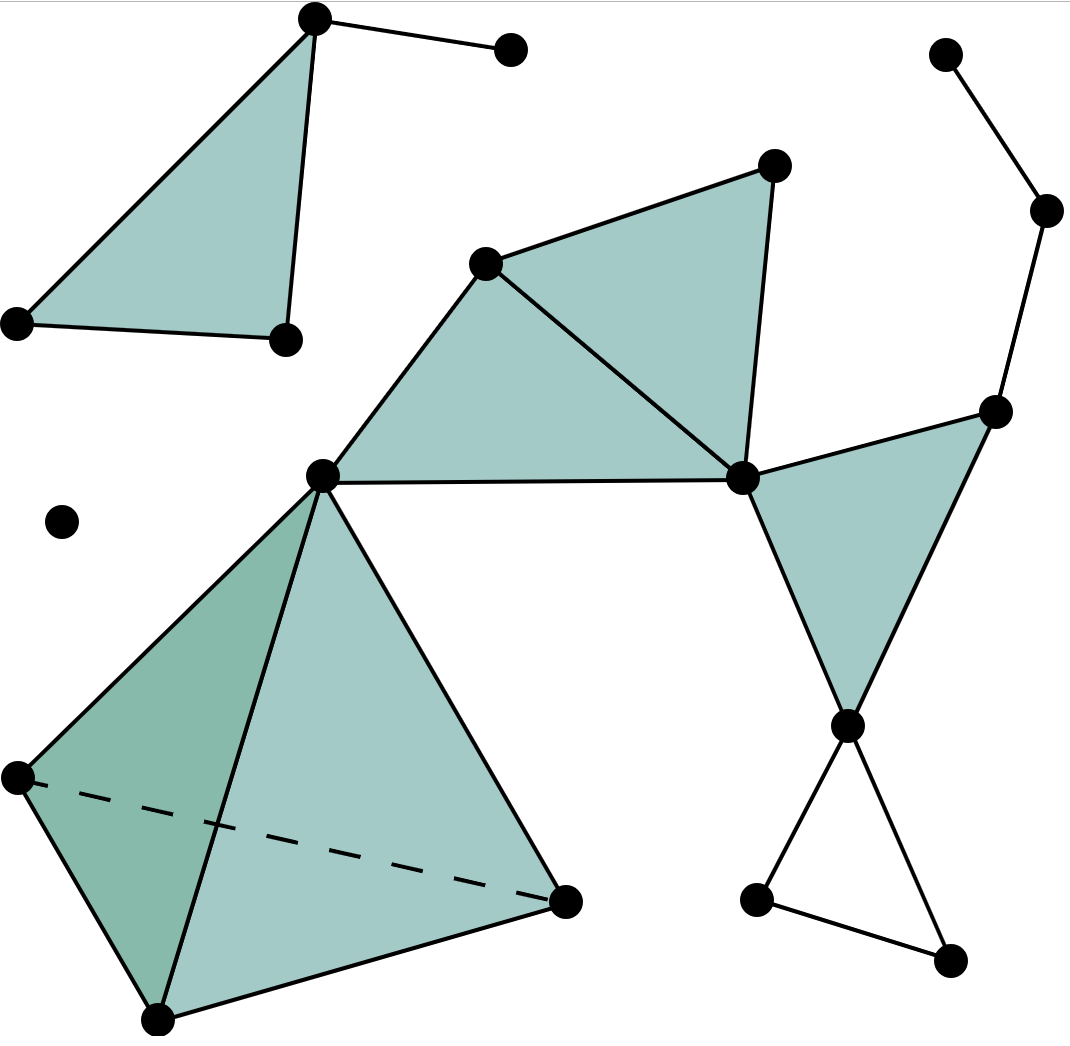
\includegraphics[width=0.2\textwidth]{SimplicialComplex.png}
\hspace{20mm}
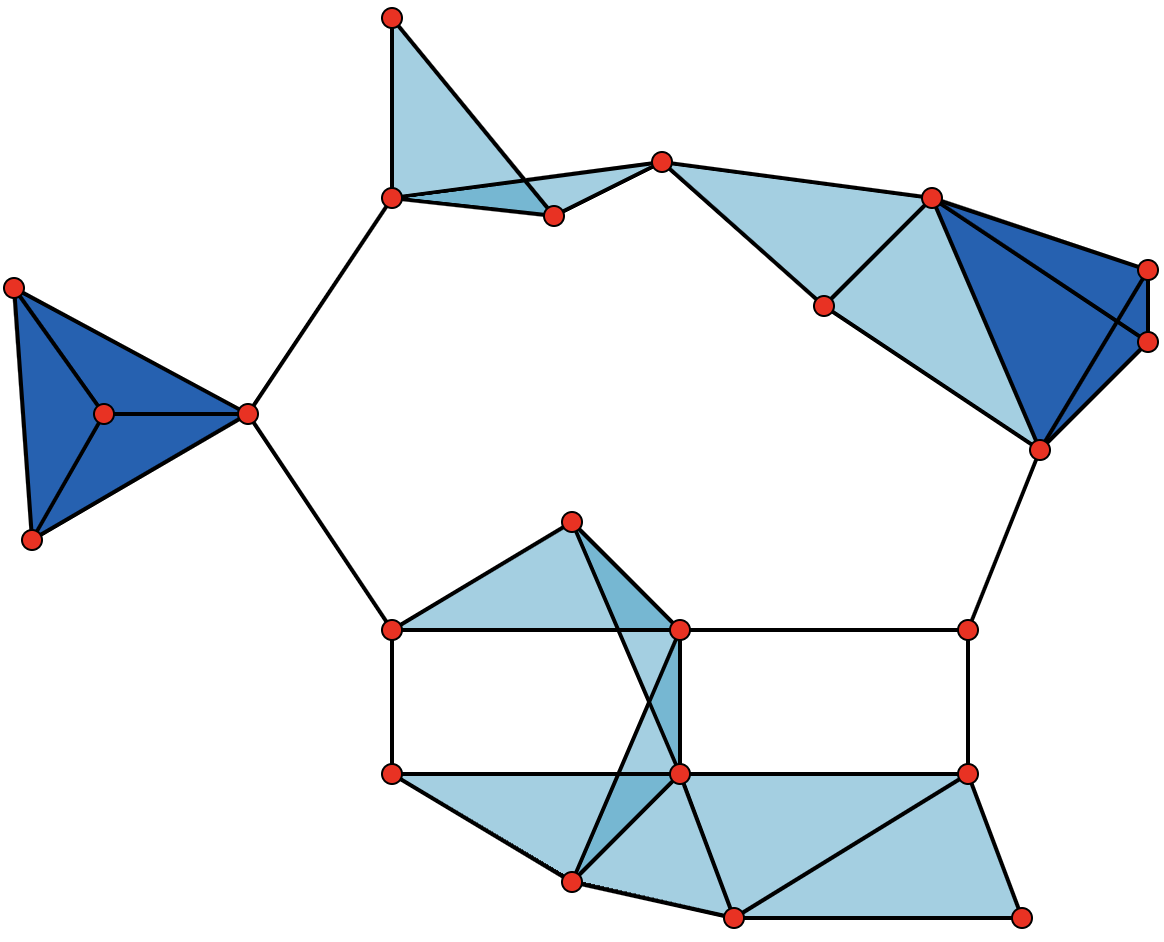
\includegraphics[width=0.25\textwidth]{CliqueComplex.png}
\caption{(Left) A simplicial complex. (Right) A clique complex.
Note the leftmost figure is not a clique complex since it has an empty triangle!
Both figures are from Wikipedia.}
\label{fig:simplicialComplex}
\end{figure}

A \emph{clique complex} is a way to build a simplicial complex on top of a graph; see for example \url{https://en.wikipedia.org/wiki/Clique\_complex}.
More specifically, let $G=(V,E)$ be a simple undirected graph (no loops or multiple edges) with $V$ the set of vertices and with $E$ the set of edges.

\begin{definition}
The \emph{clique complex $\cl(G)$} of a graph $G=(V,E)$ is the largest simplicial complex that has $V$ as its set of vertices and $E$ as its set of edges.
That is, $\cl(G)$ contains $\{v_0,\ldots,v_k\}\subseteq V$ as a simplex if $v_iv_j\in E$ (i.e.\ if $v_iv_j$ is an edge in $G$) for all $0\le i,j\le k$.
\end{definition}

\note{Notice that the clique complex of the unit disk graph is the Vietoris-Rips complex of its vertex set with $\delta = 1$, equipped with the Euclidean metric - Andrew}

Recall from Definition~\ref{def:dominated} that in a graph $G$ there is a notion of when one vertex \emph{dominates} another.
It turns out that if $u$ is a dominated vertex, then removing $u$ from $G$ doesn't affect ``the shape" of the clique complex of $G$ in any significant way!
More precisely, if $v$ is a dominated vertex, and if $G\setminus v$ is the graph obtained by removing vertex $v$, then we have a ``homotopy equivalence" of clique complexes $\cl(G)\simeq \cl(G\setminus v)$.
This means that $\cl(G)$ and $\cl(G\setminus v)$ are ``the same shape", topologically speaking.
See Figure~\ref{fig:dominatedClique}.\footnote{The ``fancy" explanation for why $\cl(G)$ and $\cl(G\setminus v)$ have the same shape, topologically speaking, is because the ``link" of $v$ (drawn in blue in Figure~\ref{fig:dominatedClique}) is contractible (it is a cone with apex $u$).}.

\begin{figure}[h]
\centering
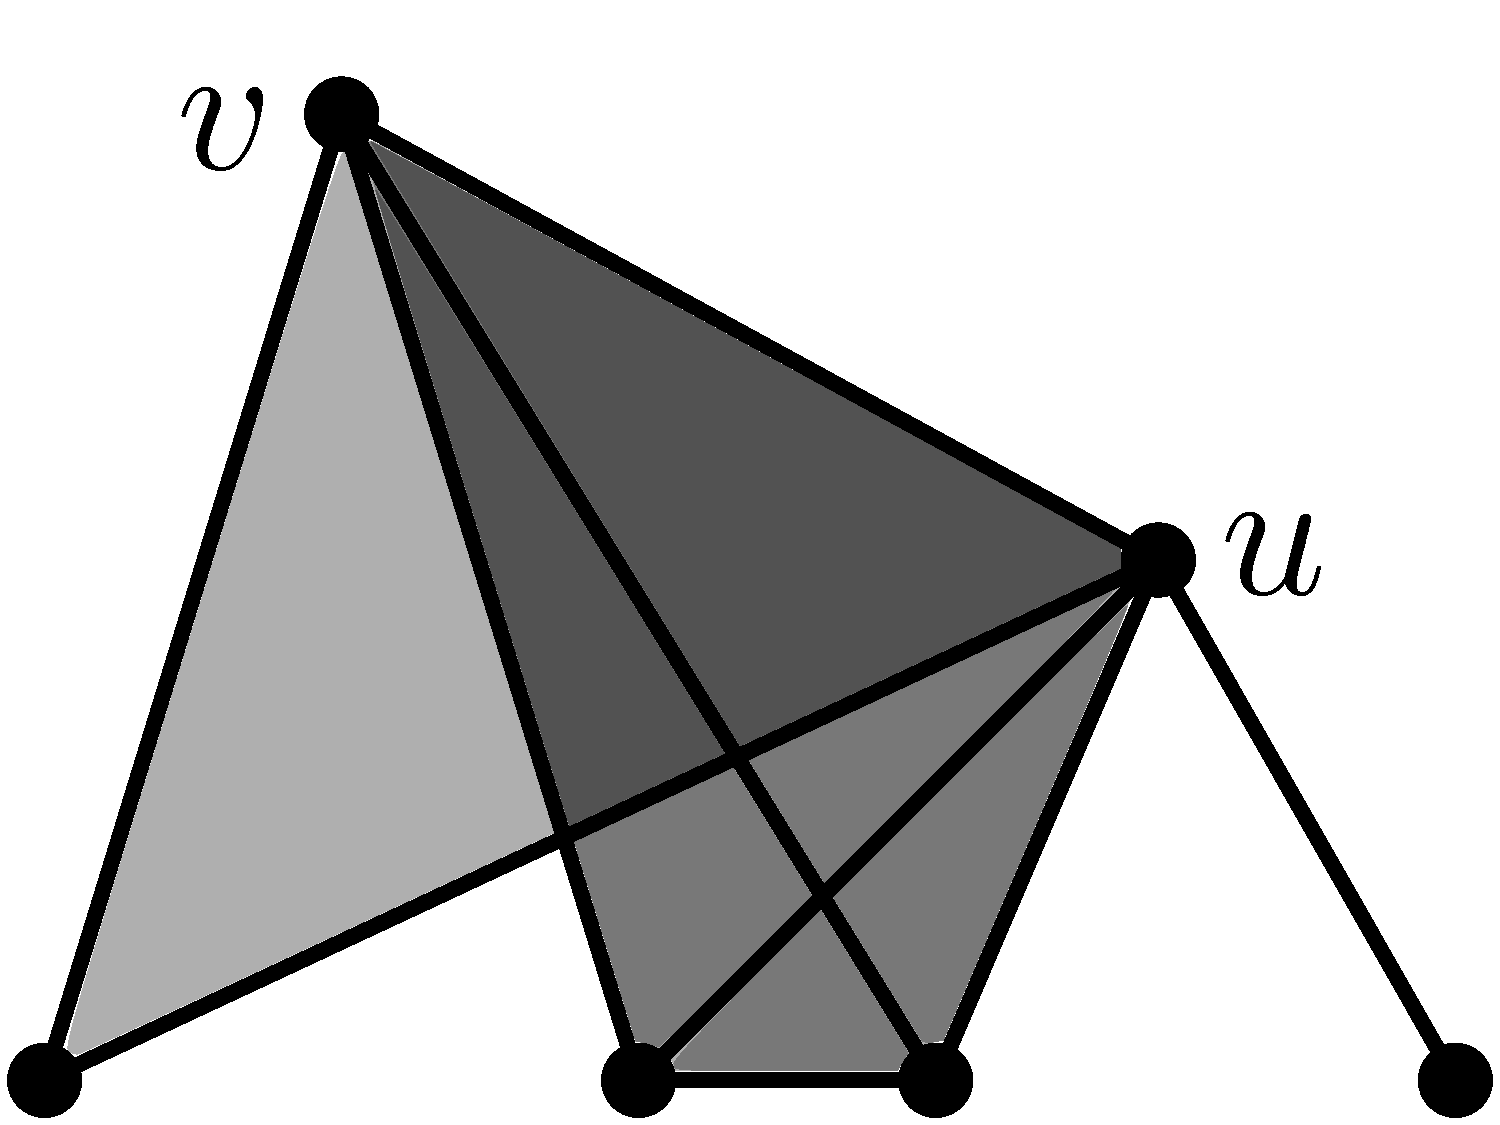
\includegraphics[width=0.2\textwidth]{Dominated2_labeled.pdf}
\hspace{20mm}
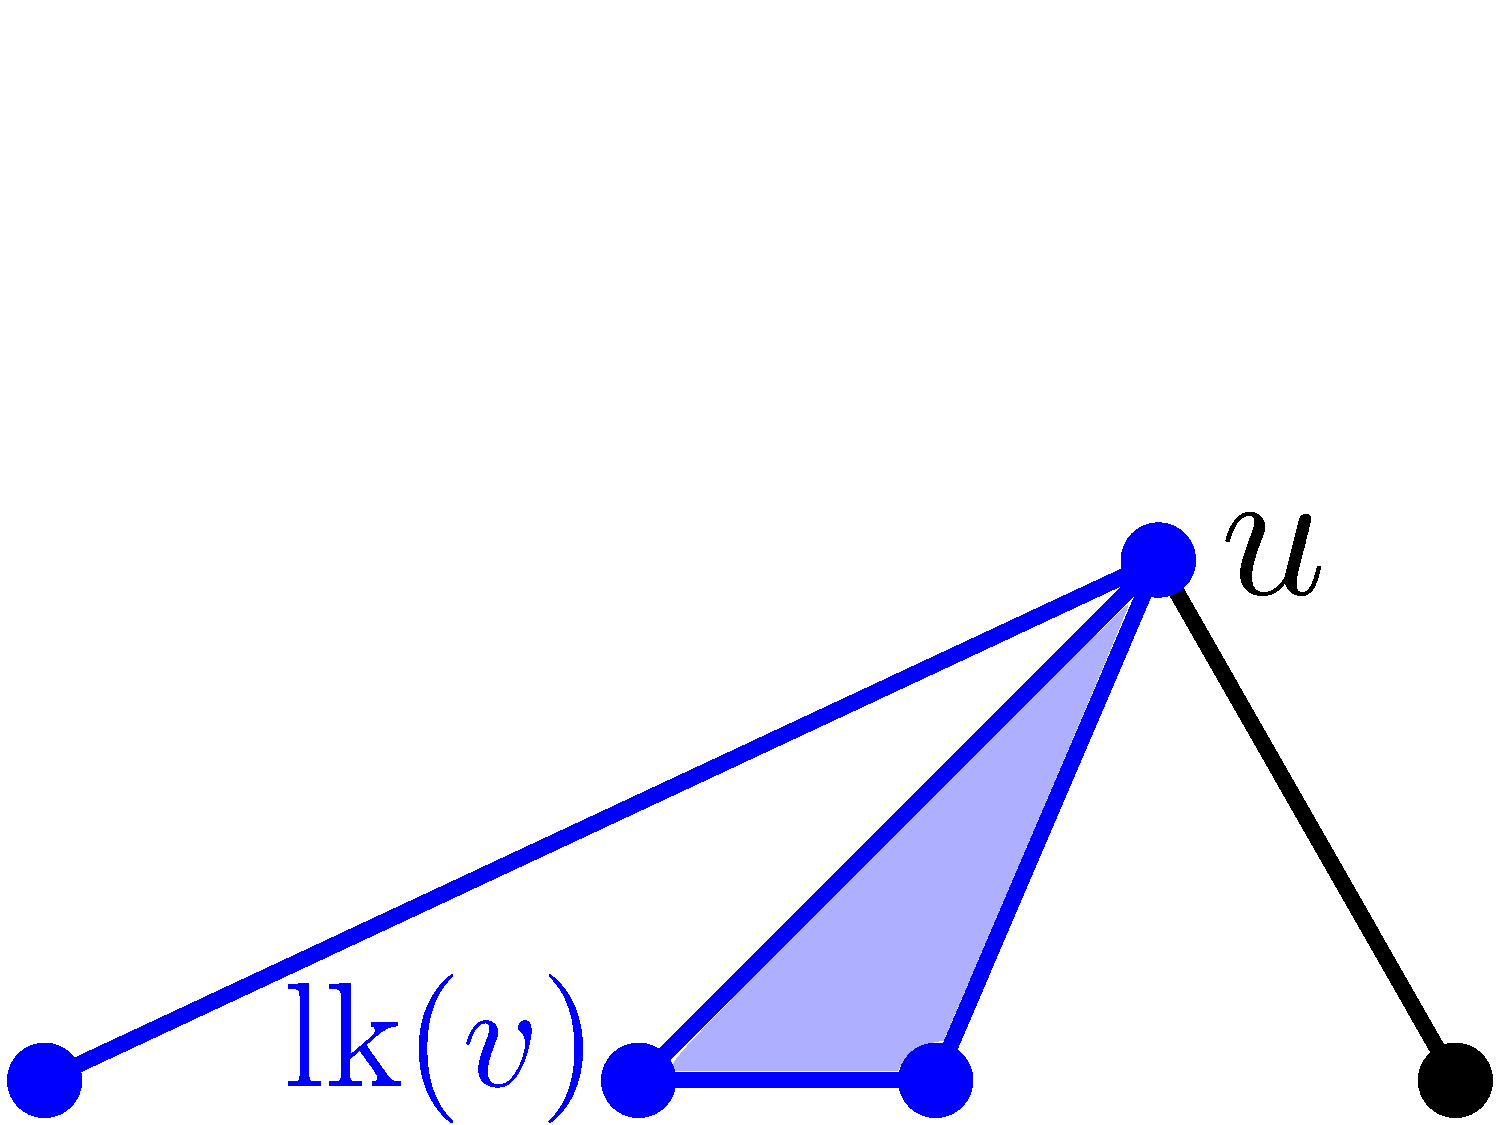
\includegraphics[width=0.2\textwidth]{Dominated4_labeled.pdf}
\caption{(Left) The clique complex $\cl(G)$. (Right) The clique complex $\cl(G\setminus v)$ after the dominated vertex $v$ has been removed. These simplicial complexes have the same shape, topologically speaking.}
\label{fig:dominatedClique}
\end{figure}

Some references for dominated vertices are \cite{BabsonKozlov2006,barmak2012strong,Matouvsek2008}, although those references are perhaps way more complicated than what we need (the notion of dominated vertices for arbitrary simplicial complexes is more complicated than that for clique complexes).


\note{How are these topological spaces defined?}



\section{Questions involving topology}

If the clique complex is ever not a wedge sum of spheres, then we have disproved an open conjecture!

If the clique complexes are always wedges of spheres, then by analyzing their cores, we may gain insight on how to prove this conjecture.

In the minimal cores that we generate, are all of the homology generators easy to interpret (using what's known on the circle)?



\section{Other notions of ``collapse" in topology}

(Besides removing dominated vertices)




\bibliographystyle{plain}
\bibliography{minimalCores}

\end{document}
